\documentclass{beamer}
\usepackage{tikz}

% internal parameters
\usetheme{Copenhagen}
\usecolortheme{default}
\setbeamertemplate{caption}[numbered]

% packages
\usepackage{graphics}
\usepackage{amsmath}
\usepackage{xcolor}
\usepackage{physics}


\title[Wobbling Motion]{New Results Concerning Collective Motion in Triaxial Nuclei}
\author[Robert POENARU]{Robert POENARU\inst{1,2}}

\institute[VFU]
{
  \inst{1}%
  Dept. of Th. Phys. @ IFIN-HH\\
  Magurele, Romania
  \and
  \inst{2}%
  Doctoral School of Physics\\
  Bucharest, Romania
}

\date{\textit{UB Faculty of Physics Meeting}\\\textit{\today}}

%------------------------------------------------------------
%The next block of commands puts the table of contents at the 
%beginning of each section and highlights the current section:
% \AtBeginSection[]
% {
%   \begin{frame}
%     \frametitle{Table of Contents}
%     \tableofcontents[currentsection]
%   \end{frame}
% }

%------------------------------------------------------------
\begin{document}
%---------------------------------------------------------
\frame{\titlepage}
\begin{frame}
  \frametitle{Table of Contents}
  \tableofcontents
\end{frame}

\section{Nuclear Shapes}
\begin{frame}{Nuclear Deformation}
\par Most of the nuclei are either \emph{spherical} or \emph{axially symmetric} in their ground-state.
\par Deformation parameter $\beta$ (\textit{Bohr, 1969}): preserves axial symmetry
\begin{figure}
  \centering
  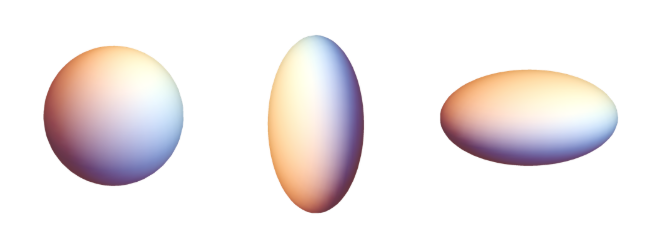
\includegraphics[width=0.99\textwidth]{Figs/nuclear_shapes.png}
  \caption{\textbf{spherical:} $\beta=0$\ \textbf{prolate:} $\beta>0$\ \textbf{oblate:} $\beta<0$}
\end{figure}
\end{frame}

\begin{frame}
  \frametitle{Nuclear Triaxiality}
  \begin{alertblock}{Non-axial shape}
    \par Deviations from symmetric shapes can occur across the chart of nuclides $\to$ \textbf{triaxial nuclei}.
    \par The triaxiality parameter $\gamma$ (\textit{Bohr, 1969}): departure from axial symmetry
  \end{alertblock}
  \begin{figure}
    \centering
    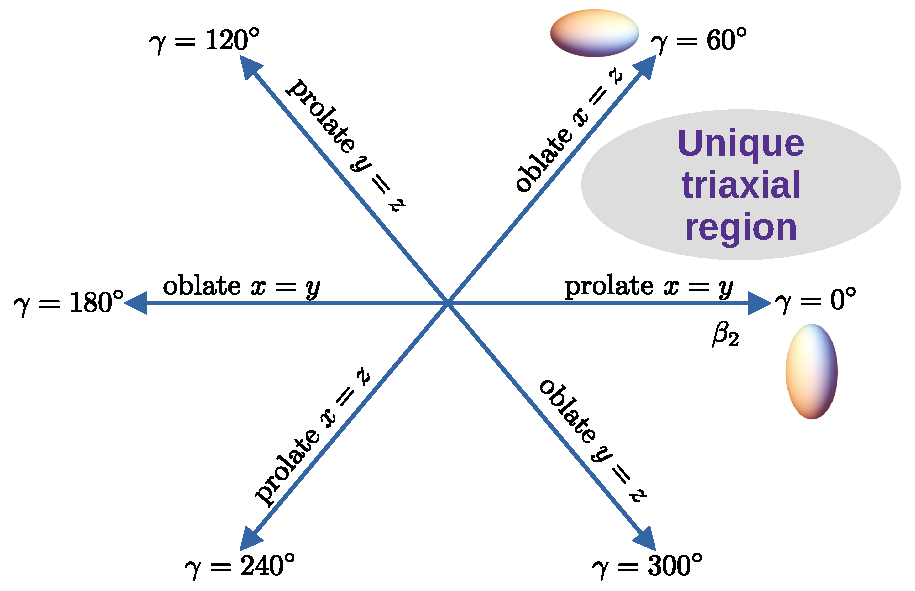
\includegraphics[scale=0.42]{Figs/nice_diagram.pdf}
    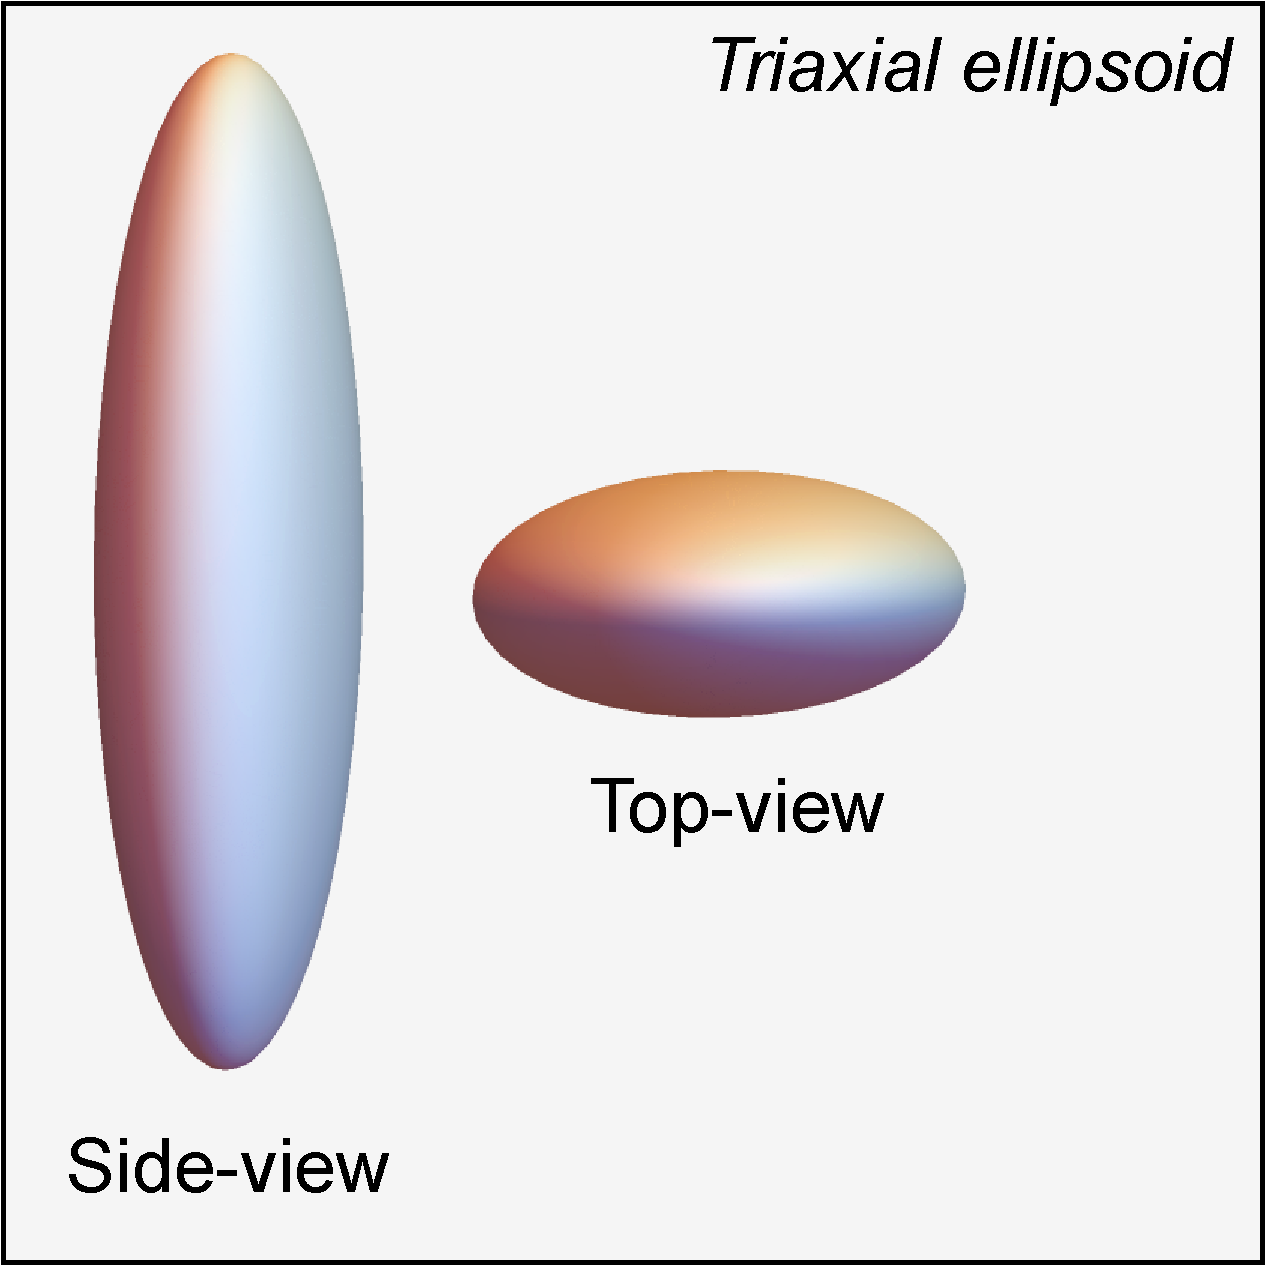
\includegraphics[scale=0.19]{Figs/triaxial-shape.pdf}
    % \caption{The $(\beta,\gamma)$ plane divided into six equivalent parts, depicting nuclear surfaces.}
  \end{figure}
\end{frame}

\begin{frame}
  \frametitle{Fingerprints for Triaxiality}
  \begin{itemize}
    \item Experimentally, stable triaxial nuclei represent a real challenge
    \item Clear signatures for confirming stable triaxiality in nuclei
    \begin{enumerate}
      \item Chiral symmetry breaking (\textit{Frauendorf, 1997})
      \item \textbf{Wobbling motion} (\textit{Bohr \& Mottelson, 1975})
    \end{enumerate}
  \end{itemize}

  \begin{block}{Wobbling Motion (WM)}
    \begin{itemize}
      \item Unique to non-axial nuclei
      \item Predicted 50 years ago for even-$A$ nuclei
      \item First experimental evidence for $^{163}$Lu (\textit{Ødegård}, 2001)
      \item Currently: confirmed wobblers within the mass regions $A\approx[100,130,160,180]$.
    \end{itemize}
  \end{block}
\end{frame}

\begin{frame}
  \frametitle{Experimental Evidence}
  \begin{figure}
    \centering
    \begin{minipage}{.5\textwidth}
      \begin{figure}
        \centering
        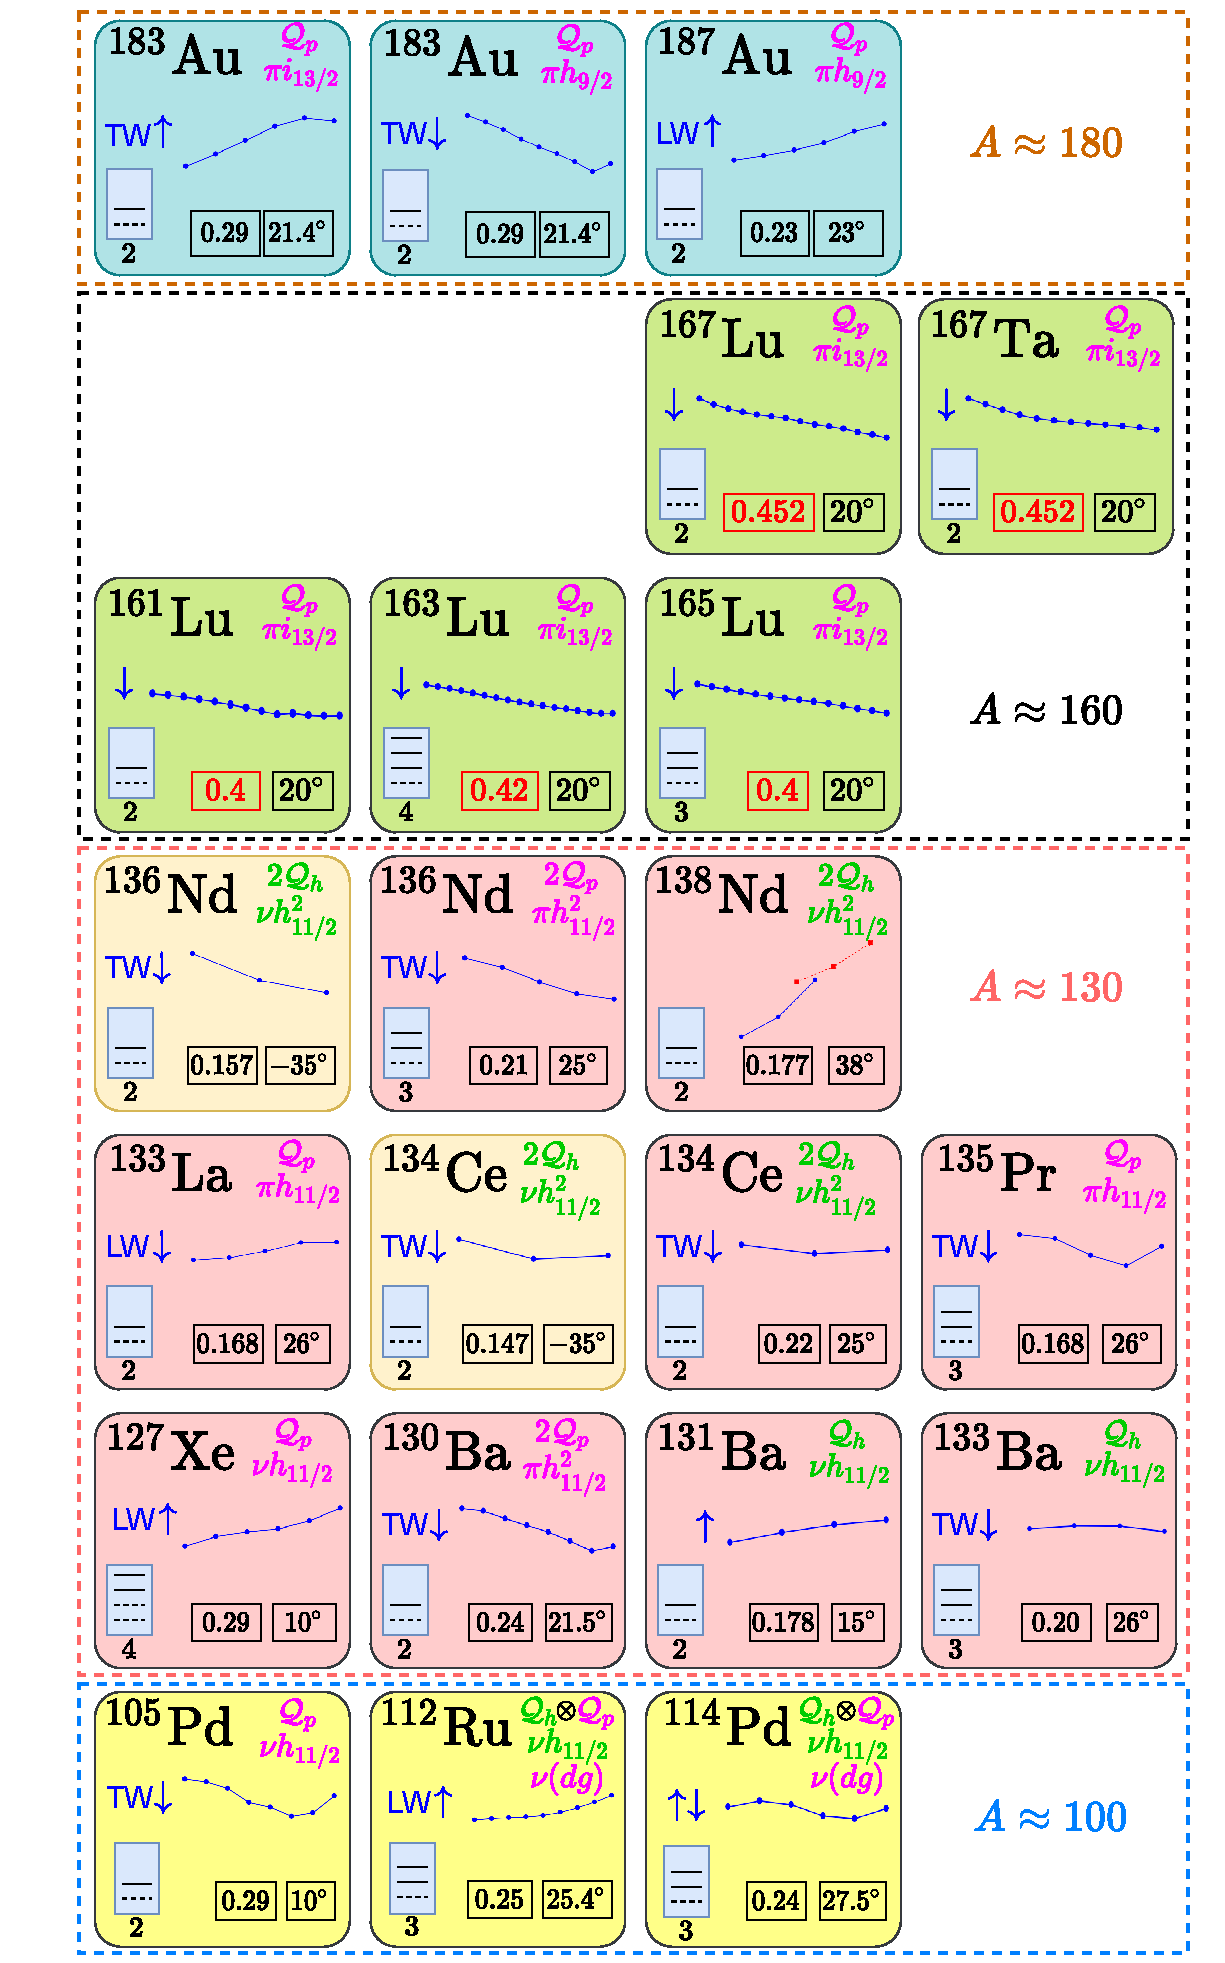
\includegraphics[scale=0.22]{Figs/wobblers-chart.pdf}
      \end{figure}
    \end{minipage}%
    \begin{minipage}{.5\textwidth}
      \par Wobbling nuclei (up to date)
      \par \textit{Poenaru, 2022, in progress}
    \end{minipage}
    \end{figure}
\end{frame}

\begin{frame}
  \frametitle{Energy of Deformed Nuclei}
    \begin{block}{Collective Motion}
      \begin{itemize}
        \item A nucleus - \emph{droplet} - can generate angular momentum from the rotation and vibration of the droplet itself
        \item Each individual nucleon contributes to the total angular momentum $\rightarrow$ \emph{collectiveness}
      \end{itemize}
    \end{block}
    \begin{figure}
      \centering
      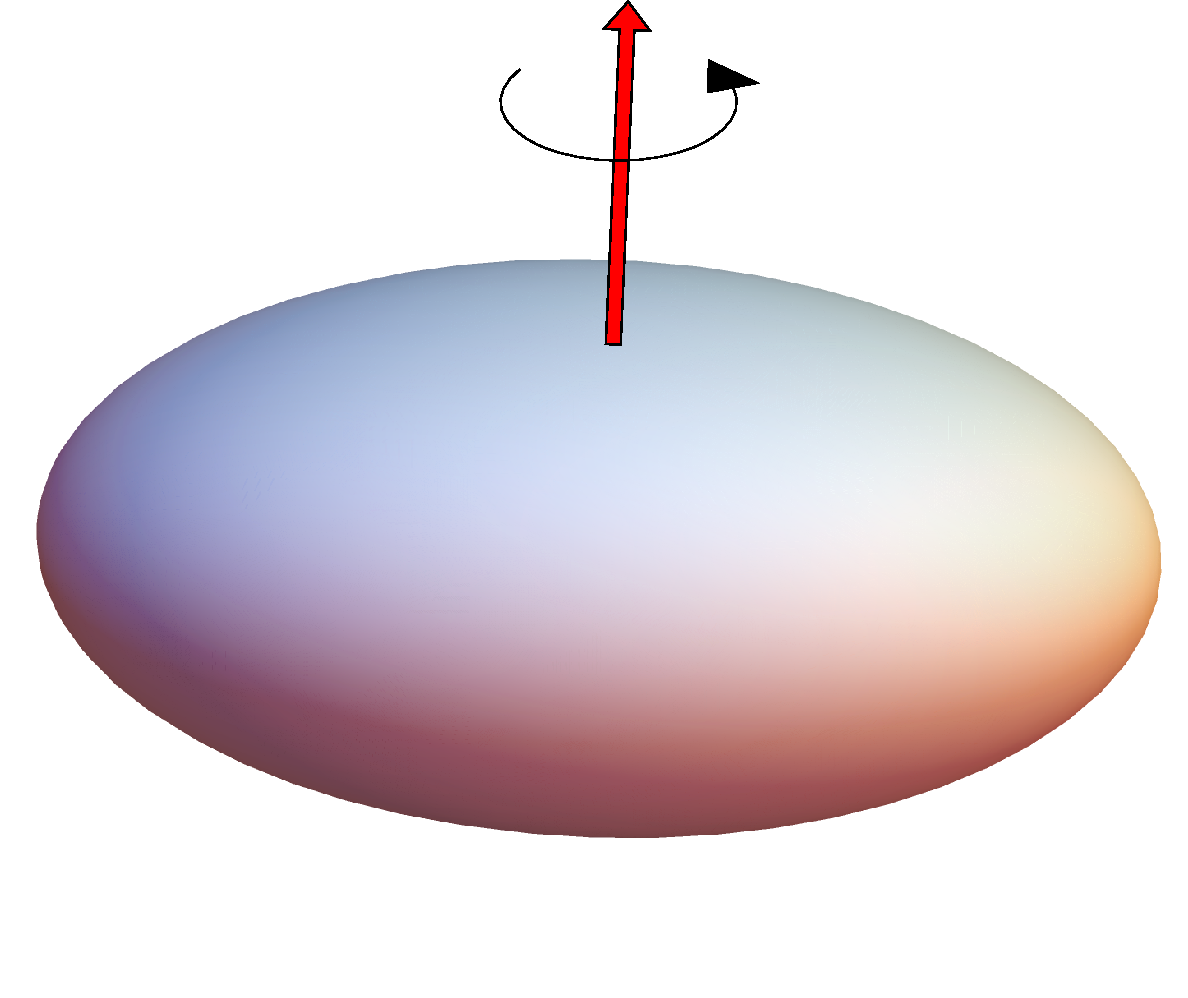
\includegraphics[scale=0.26]{Figs/collective-rotation.pdf}
    \end{figure}
\end{frame}

\begin{frame}
  \frametitle{Triaxial Rotor Energy}
  \begin{itemize}
    \item A triaxial nucleus can rotate about any of the three axes
    \item Rotation about the axis with \textbf{the largest moment of inertia} (MOI) is energetically the most favorable: $E_\text{rot}\propto\frac{\hbar^2}{2\mathcal{I}_\text{max}}I(I+1 )$
    \item MOI anisotropy $\rightarrow$ the \emph{main rotation} around $\mathcal{J}_\text{max}$ is disturbed by the other two axes $\rightarrow$ {\color{red}\emph{total motion of the rotating nucleus has an oscillating behavior}}
  \end{itemize}
  \begin{figure}
    \centering
    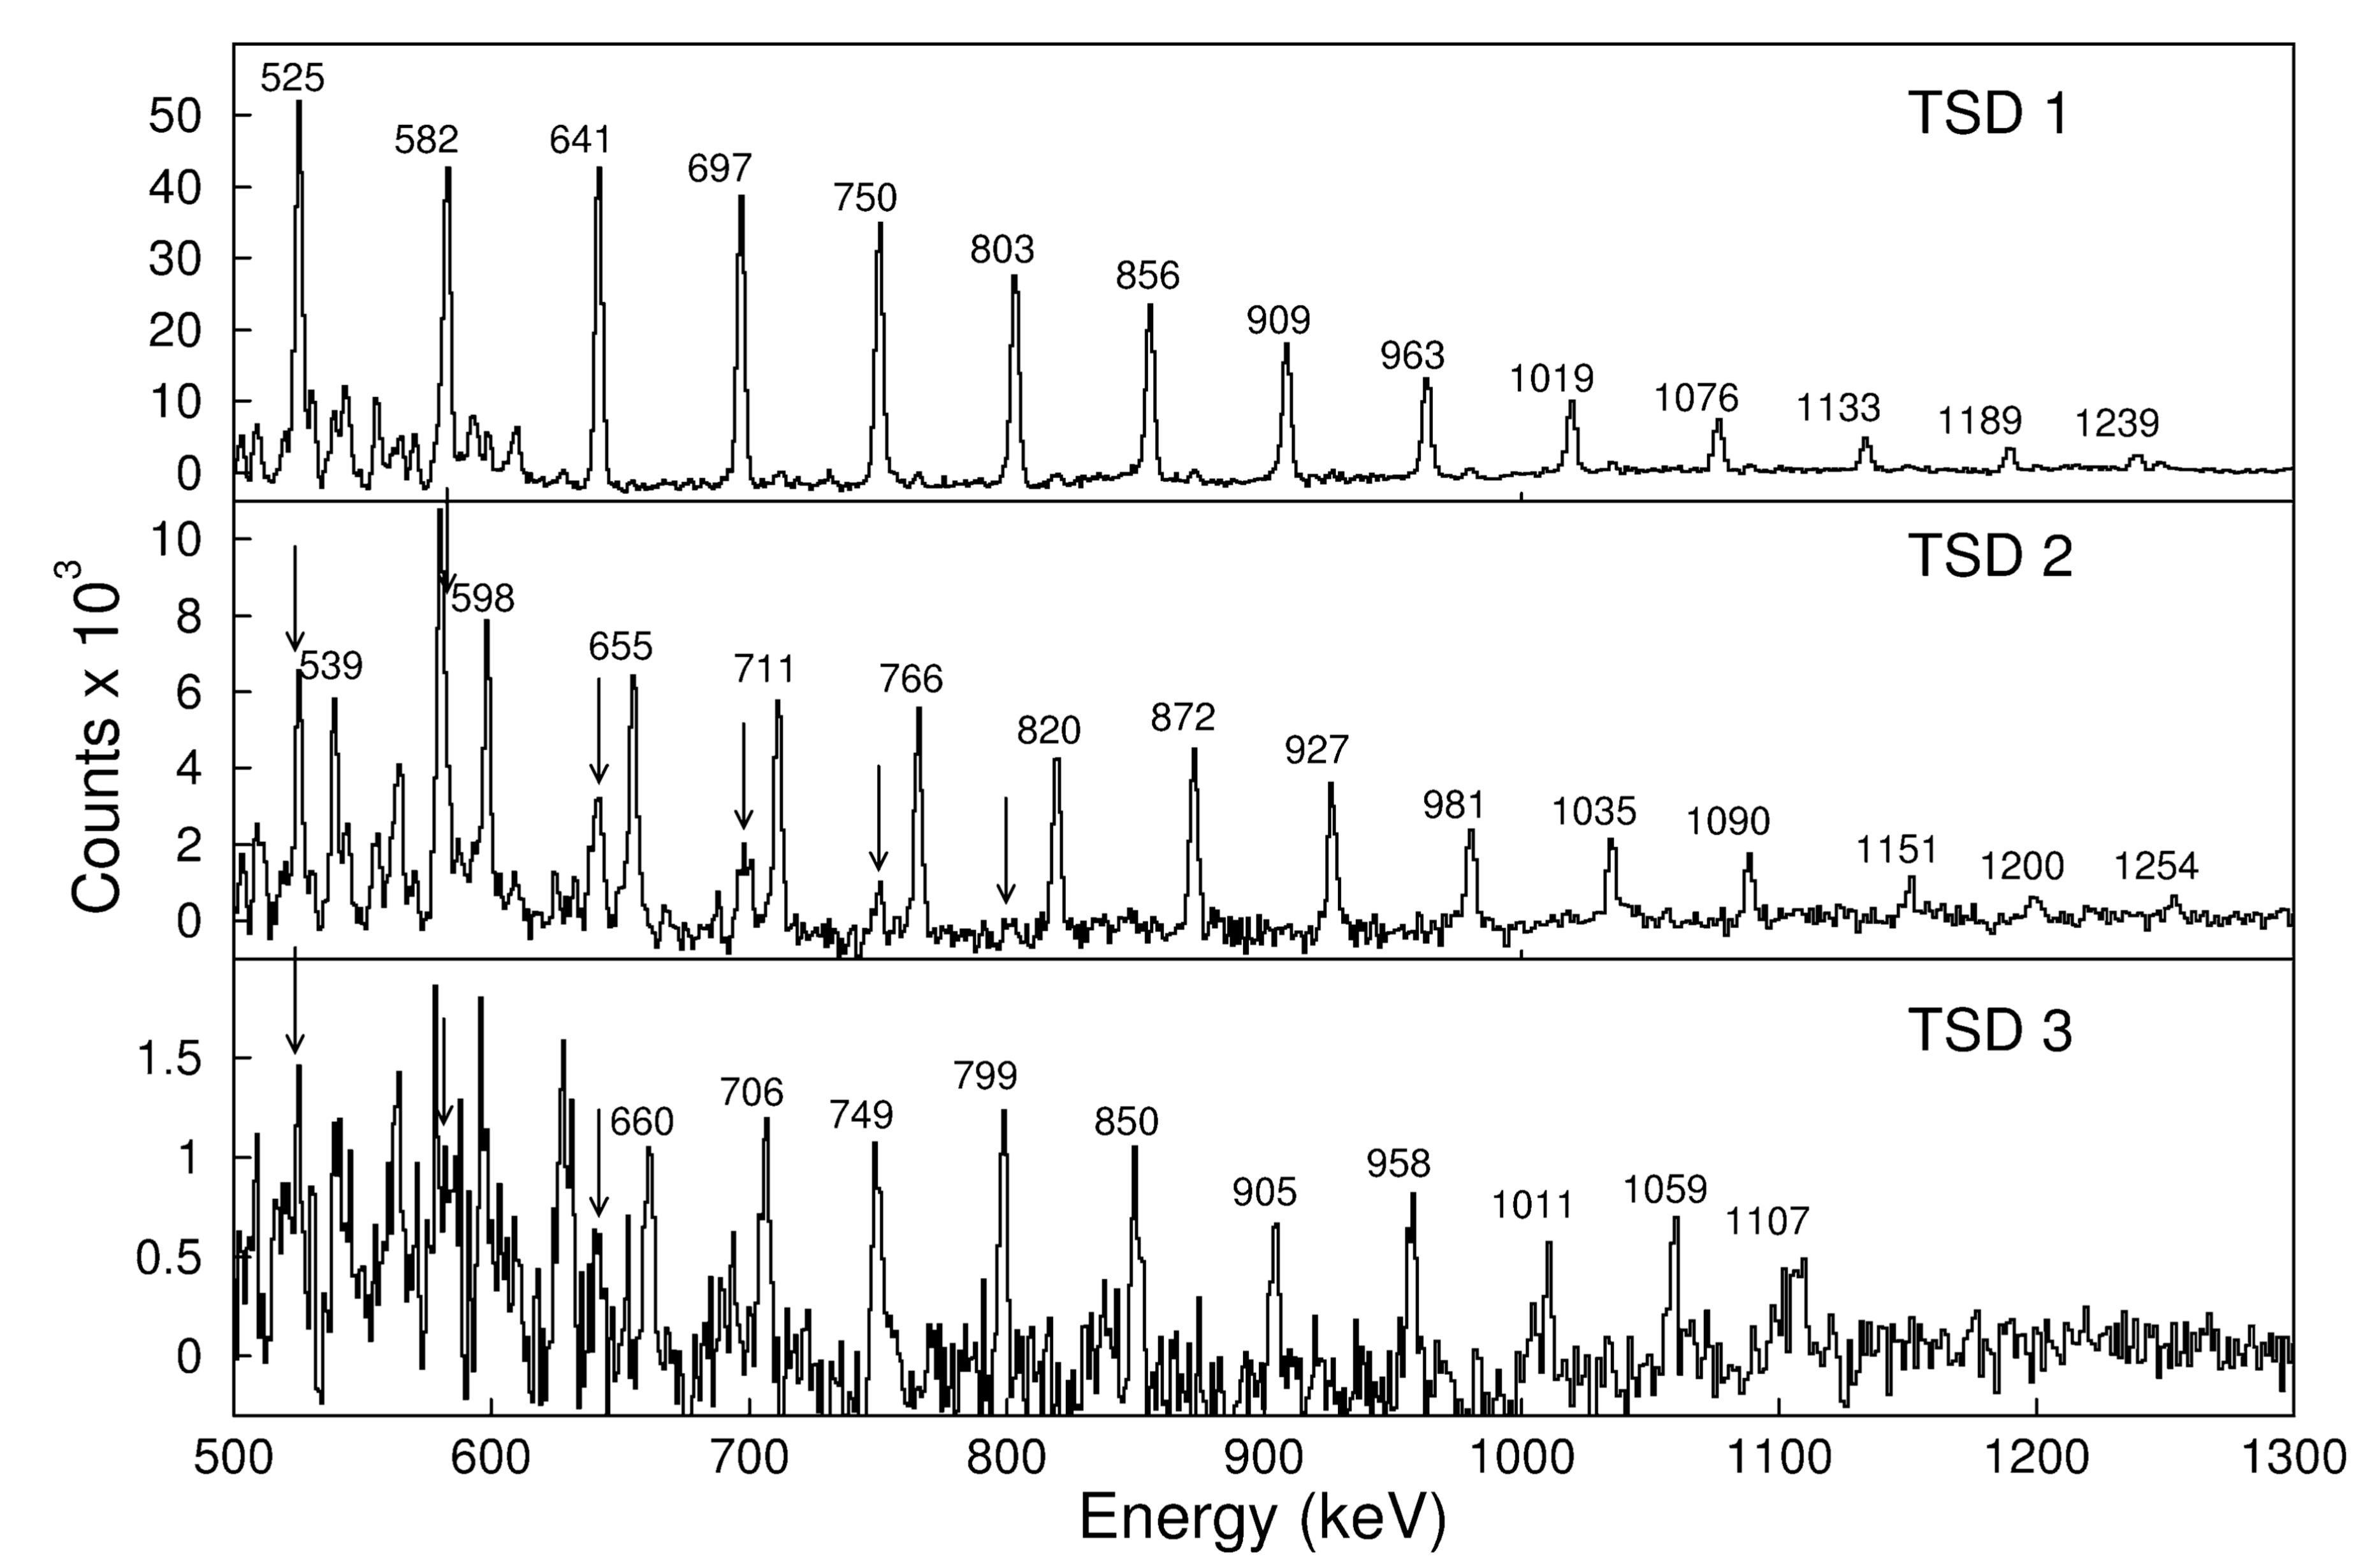
\includegraphics[scale=0.1]{Figs/collective-spectra.pdf}
    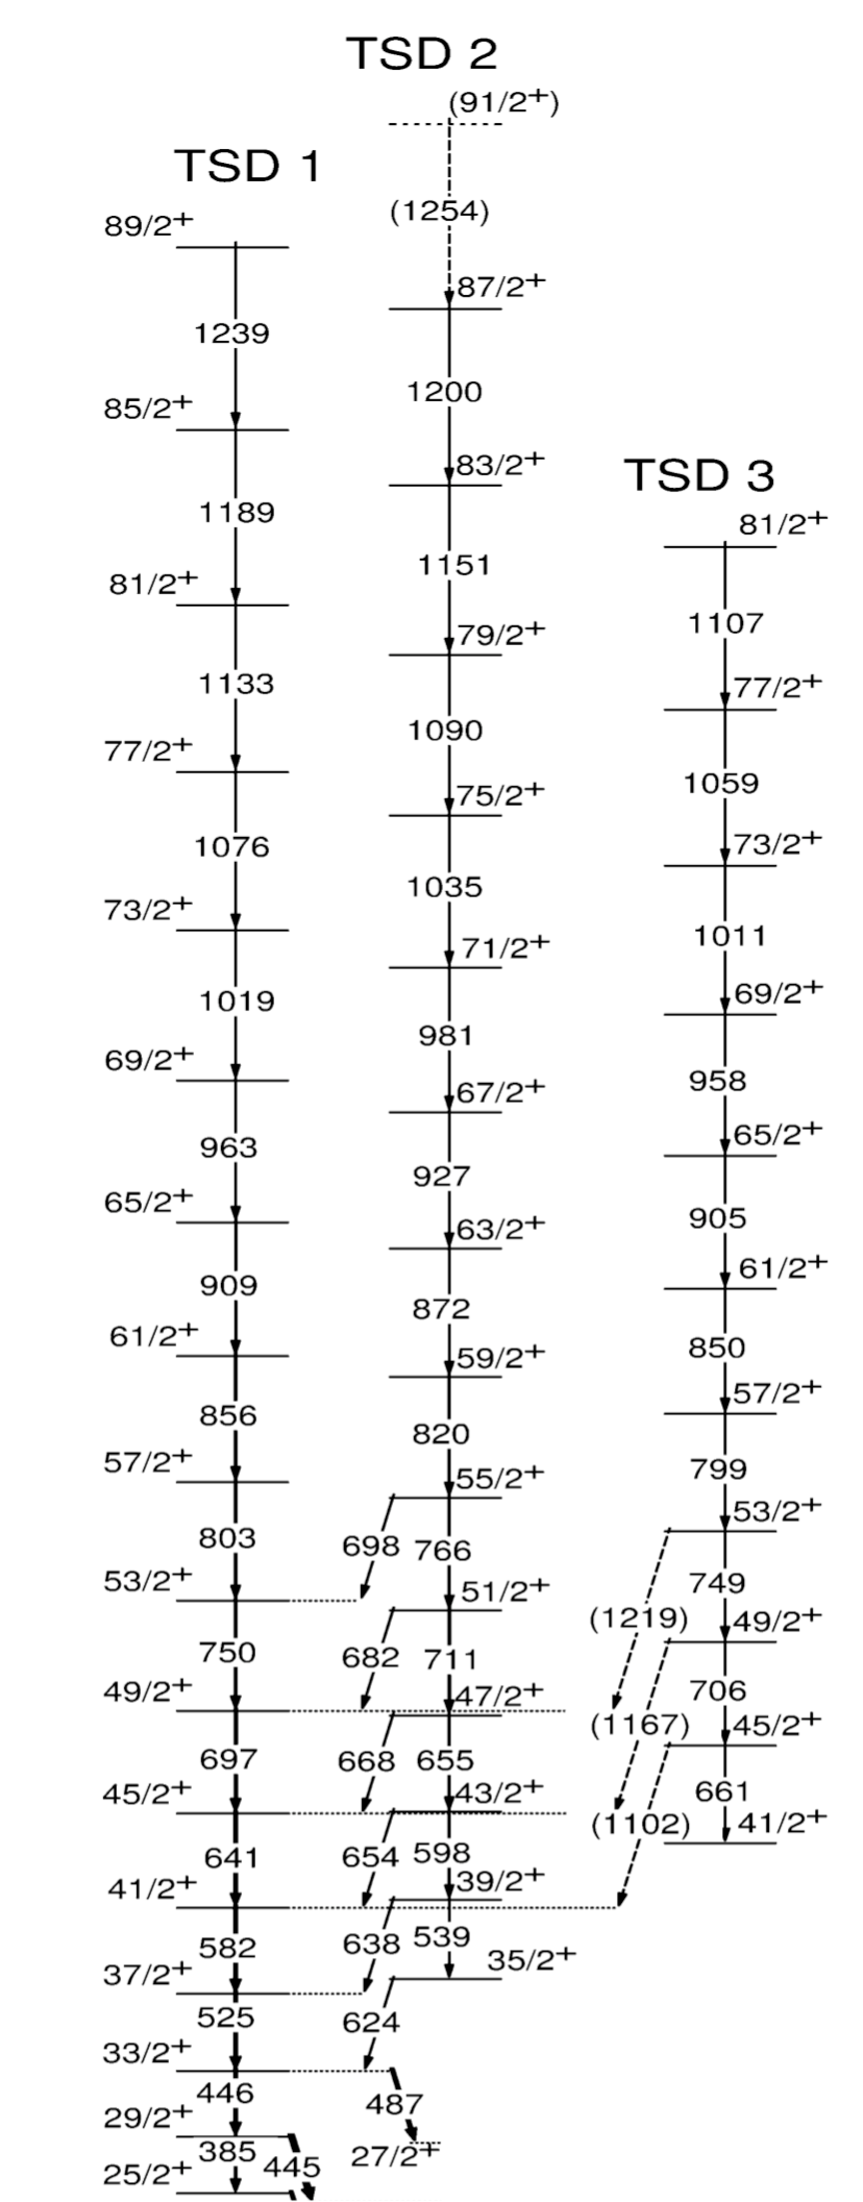
\includegraphics[scale=0.115]{Figs/collective-levels.pdf}
  \end{figure}
\end{frame}

\begin{frame}
  \frametitle{Wobbling Motion}
\begin{itemize}
  \item Total angular momentum $\mathbf{I}$ disaligned w.r.t. body-fixed axes
  \item The a.m. \textbf{precesses} and \textbf{wobbles} around the axis with $\mathcal{J}_\text{max}$
  \item The precession of $\mathbf{I}$ can increase by \textbf{tilting} 
  \item Tilting by an energy quanta $\sim$ \emph{vibrational character} $\rightarrow$ \textbf{wobbling phonon} $n_w=0,1,2...$
\end{itemize}
  \begin{figure}
    \centering
    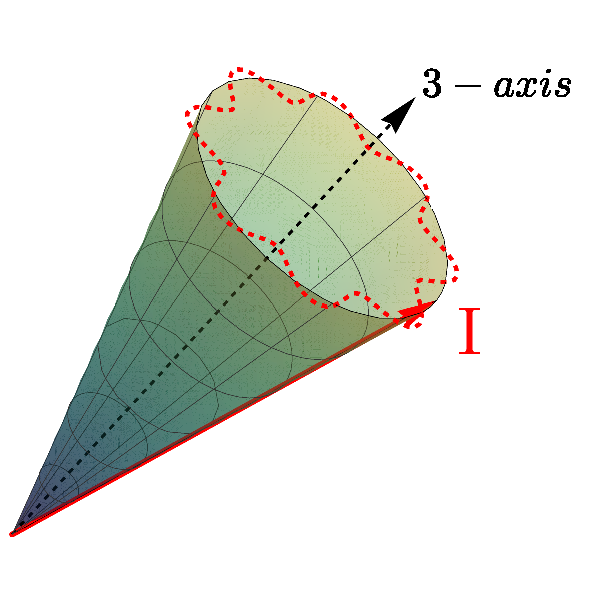
\includegraphics[scale=0.4]{Figs/precessional_cone_2.pdf}
    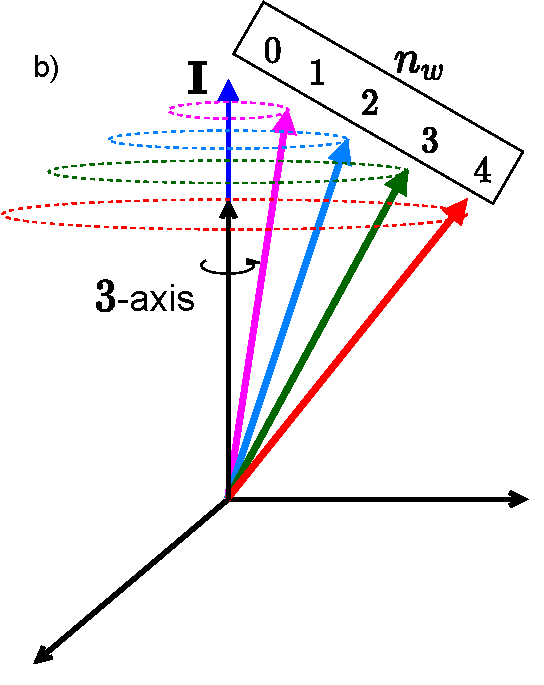
\includegraphics[scale=0.35]{Figs/wobbling_n_schematic-2.pdf}
  \end{figure}

\end{frame}

%---------------------------------------------------------
\end{document}
%---------------------------------------------------------

% \begin{frame}
%   \frametitle{Highlighting text}
  
%   In this slide, some important text will be
%   \alert{highlighted} because it's important.
%   Please, don't abuse it.
  
%   \begin{block}{Remark}
%     Sample text
%   \end{block}
  
%   \begin{alertblock}{Important theorem}
%     Sample text in red box
%   \end{alertblock}
  
%   \begin{examples}
%     Sample text in green box. The title of the block is ``Examples".
%   \end{examples}
% \end{frame}